\section {Implementation and Technical Notes}

Python 3.6 was used to code, with modularity of components being the main focus. 

The code has been split into logical modules:
\begin{itemize}
\item \textbf{model_lib.py}: defines the MNIST model.
\item \textbf{mnist_eager.py}: trains the MNIST model with \textit{tf eager execution}.
\item  \textbf{README.md }: Contains relevant code documentation.
\end{itemize}


\section {Question 1}

We use \textit{tensorflow eager} to train the MNIST CNN Model of the following architecture:

\begin{lstlisting}
_________________________________________________________________
Layer (type)                 Output Shape              Param #   
=================================================================
reshape (Reshape)            (None, 1, 28, 28)         0         
_________________________________________________________________
conv2d (Conv2D)              (None, 32, 28, 28)        320       
_________________________________________________________________
max_pooling2d (MaxPooling2D) multiple                  0         
_________________________________________________________________
conv2d_1 (Conv2D)            (None, 32, 14, 14)        9248      
_________________________________________________________________
flatten (Flatten)            (None, 1568)              0         
_________________________________________________________________
dense (Dense)                (None, 500)               784500    
_________________________________________________________________
dropout (Dropout)            (None, 500)               0         
_________________________________________________________________
dense_1 (Dense)              (None, 10)                5010      
=================================================================
Total params: 799,078
Trainable params: 799,078
Non-trainable params: 0
_________________________________________________________________
\end{lstlisting}

The code to train the model is:

\begin{lstlisting}
python3 mnist/mnist_eager.py
\end{lstlisting}

\begin{itemize}
\item Learning rate of $1e-4$, with SGD momentum was used as the optimiser.
\item We periodically run evaluation post an epoch. The files are recorded as tensorboard events.
\item Logs are stored at \textit{/tmp/tensorflow/mnist}, with seperate directories for \textit{train},\textit{eval},\textit{occlusion},\textit{filters},\textit{activations} and \textit{adversarial attacks}.
\end{itemize}


We use tensorboard for logs, which can be viewed by:
\begin{lstlisting}
tensorboard --log_dir /tmp/tensorflow/mnist
\end{lstlisting}

We report a test accuracy of $99.11$, and with the cross entropy loss well below $0.03$.

\subsection{Accuracy and Loss curves}

\begin{figure}[ht]
\centering
%%\includegraphics[angle=0,width=0.8\textwidth]{Figure_1.png}
\caption{Accuracy Loss curves for \textbf{MNIST CNN}}
\end{figure}

\subsection {Code Blocks (model definition)}
\begin{lstlisting}
def create_model(data_format='channels_first'):
    """Model to recognize digits in the MNIST dataset.

    Args:
    * data_format: NHWC or NCHW. Prefer latter for CPUs, former for GPUs.

    Returns:
      A tf.keras.Model.
    """
    if data_format == 'channels_first':
        input_shape = [1, 28, 28]
    else:
        assert data_format == 'channels_last'
        input_shape = [28, 28, 1]

    l = tf.keras.layers
    max_pool = l.MaxPooling2D(
        (2, 2), (2, 2), padding='same', data_format=data_format)
    # The model consists of a sequential chain of layers, so tf.keras.Sequential
    # (a subclass of tf.keras.Model) makes for a compact description.
    return tf.keras.Sequential(
        [
            l.Reshape(
                target_shape=input_shape,
                input_shape=(28 * 28,)),
            l.Conv2D(
                32,
                3,
                padding='same',
                data_format=data_format,
                activation=tf.nn.relu),
            max_pool,
            l.Conv2D(
                32,
                3,
                padding='same',
                data_format=data_format,
                activation=tf.nn.relu),
            max_pool,
            l.Flatten(),
            l.Dense(500, activation=tf.nn.relu),
            l.Dropout(0.4),
            l.Dense(10)
        ])
\end{lstlisting}

We run the list of properties for all possible GPU's present in the given machine.

\bigskip

\subsection{Sample Outputs}

\begin{figure}[h]
\begin{subfigure}
\centering

\includegraphics[angle=0,width=0.4\textwidth]{assign-2/logs/0.png}
\caption{Sample Output: label 0, prediction 0, probability 0.992}
\end{subfigure}
\begin{subfigure}
\centering
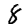
\includegraphics[angle=0,width=0.4\textwidth]{assign-2/logs/8.png}
\caption{Sample Output: label 8, prediction 8, probability 0.873}
\end{subfigure}
\end{figure}

\section{Question 2}

Visualising Filters and Activations:


\begin{figure}[h]
\begin{subfigure}
\centering

\includegraphics[angle=0,width=0.4\textwidth]{assign-2/logs/0.png}
\caption{Sample Output: label 0, prediction 0, probability 0.992}
\end{subfigure}
\begin{subfigure}
\centering
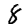
\includegraphics[angle=0,width=0.4\textwidth]{assign-2/logs/8.png}
\caption{Sample Output: label 8, prediction 8, probability 0.873}
\end{subfigure}
\end{figure}